\section{Leitungen}

\subsection{Leitungsparameter}

\subsubsection{Doppelleitung:}
\[
    a = \text{Leiter Radius} \qquad d = \text{Abstand zw. den Leitern} \\
\]

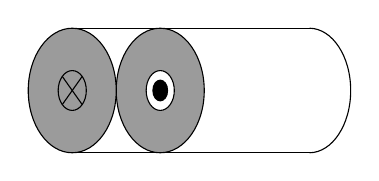
\begin{tikzpicture}[x=0.75pt,y=0.75pt,yscale=-1,xscale=1]
%Shape: Ellipse  
\draw  [fill={rgb, 255:red, 155; green, 155; blue, 155 }  ,fill opacity=1 ] (256.6,107.4) .. controls (256.6,90.83) and (266.09,77.4) .. (277.8,77.4) .. controls (289.51,77.4) and (299,90.83) .. (299,107.4) .. controls (299,123.97) and (289.51,137.4) .. (277.8,137.4) .. controls (266.09,137.4) and (256.6,123.97) .. (256.6,107.4) -- cycle ;
%Shape: Ellipse  
\draw  [fill={rgb, 255:red, 155; green, 155; blue, 155 }  ,fill opacity=1 ] (214.2,107.4) .. controls (214.2,90.83) and (223.69,77.4) .. (235.4,77.4) .. controls (247.11,77.4) and (256.6,90.83) .. (256.6,107.4) .. controls (256.6,123.97) and (247.11,137.4) .. (235.4,137.4) .. controls (223.69,137.4) and (214.2,123.97) .. (214.2,107.4) -- cycle ;
%Straight Lines  
\draw    (235.4,77.4) -- (284.77,77.4) ;
%Straight Lines  
\draw    (235.4,137.4) -- (284.77,137.4) ;
%Shape: Arc  
\draw  [draw opacity=0] (349.76,137.4) .. controls (360.71,137.28) and (369.56,123.89) .. (369.56,107.4) .. controls (369.56,90.92) and (360.73,77.55) .. (349.8,77.4) -- (349.61,107.4) -- cycle ; \draw   (349.76,137.4) .. controls (360.71,137.28) and (369.56,123.89) .. (369.56,107.4) .. controls (369.56,90.92) and (360.73,77.55) .. (349.8,77.4) ;  
%Straight Lines  
\draw    (284.95,77.4) -- (349.8,77.4) ;
%Straight Lines  
\draw    (284.95,137.4) -- (349.8,137.4) ;
%Flowchart: Summing Junction  
\draw   (228.62,107.4) .. controls (228.62,102.1) and (231.65,97.8) .. (235.4,97.8) .. controls (239.15,97.8) and (242.18,102.1) .. (242.18,107.4) .. controls (242.18,112.7) and (239.15,117) .. (235.4,117) .. controls (231.65,117) and (228.62,112.7) .. (228.62,107.4) -- cycle ; \draw   (230.6,100.61) -- (240.2,114.19) ; \draw   (240.2,100.61) -- (230.6,114.19) ;
%Shape: Ellipse  
\draw  [fill={rgb, 255:red, 255; green, 255; blue, 255 }  ,fill opacity=1 ] (271.02,107.4) .. controls (271.02,102.1) and (274.05,97.8) .. (277.8,97.8) .. controls (281.55,97.8) and (284.58,102.1) .. (284.58,107.4) .. controls (284.58,112.7) and (281.55,117) .. (277.8,117) .. controls (274.05,117) and (271.02,112.7) .. (271.02,107.4) -- cycle ;
%Shape: Ellipse  
\draw  [fill={rgb, 255:red, 0; green, 0; blue, 0 }  ,fill opacity=1 ] (274.27,107.4) .. controls (274.27,104.64) and (275.85,102.4) .. (277.8,102.4) .. controls (279.75,102.4) and (281.33,104.64) .. (281.33,107.4) .. controls (281.33,110.16) and (279.75,112.4) .. (277.8,112.4) .. controls (275.85,112.4) and (274.27,110.16) .. (274.27,107.4) -- cycle ;
\end{tikzpicture}

{\renewcommand*{\arraystretch}{0.2}
    \begin{tabularx}{0.5\columnwidth}{|X|}
        \hline
        \[R  = \frac{1}{\pi a\delta\sigma_c}\]              \\
        \hline
        \[L = \frac{\mu}{\pi} \cosh^{-1}\frac{d}{2a}\]      \\
        \hline
        \[G = \frac{\pi\sigma}{\cosh^{-1}(^d/_{2a})}\]      \\
        \hline
        \[C = \frac{\pi\varepsilon}{\cosh^{-1}(^d/_{2a})}\] \\
        \hline
    \end{tabularx}}

\subsubsection{Koaxial Leitung}
\[
    a = \text{innen Radius} \qquad b = \text{außen Radius} \\
\]
\begin{align*}
    \vec{H}(r, z) & = \frac{I}{2\pi r}\cdot e^{-j\beta z}\cdot\vec{e}_\varphi                    \\
    \vec{E}(r, z) & = \frac{I}{2\pi r}\cdot Z_F\cdot e^{-j\beta z} \cdot\vec{e}_r                \\
                  & = \frac{\hat{U}}{r \cdot\ln{(^{2b}/_{2a})}}\cdot e^{-j\beta z}\cdot\vec{e}_r
\end{align*}

\begin{tikzpicture}
    \tikzset{cross/.style={cross out, draw=black, minimum size=2*(#1-\pgflinewidth), inner sep=0pt, outer sep=0pt},
        %     %default radius will be 1pt. 
        cross/.default={3.5pt}}

        %Außenleiter
        \draw[-](-0.53,0.53)--(0.97,2.03);
        \draw[-](0.53,-0.53)--(1.63,0.57);

        \draw[-](0,0) circle (0.75);

        %Innenleiter
        \draw[-](-0.106,0.106)--(0.41,0.622);
        \draw[-](0.106,-0.106)--(0.622,0.41);

        \draw[-](0,0) circle (0.15);
        \draw(0,0) node [cross] {};

\end{tikzpicture}

{\renewcommand*{\arraystretch}{0.2}
    \begin{tabularx}{0.5\columnwidth}{|X|}
        \hline
        \[R=\frac{1}{2\pi\delta\sigma_c}\left[\frac{1}{a}+\frac{1}{b}\right]\] \\
        \hline
        \[L=\frac{\mu}{2\pi}\ln\frac{b}{a}\]                                   \\
        \hline
        \[G=\frac{2\pi\sigma}{\ln(^b/_a)}\]                                    \\
        \hline
        \[C=\frac{2\pi\varepsilon}{\ln(^b/_a)}\]                               \\
        \hline
    \end{tabularx}}

\subsubsection{Parallele Platten}
\[
    w  = \text{Platten Breite} \qquad d  = \text{Abstand zw. Platten}
\]

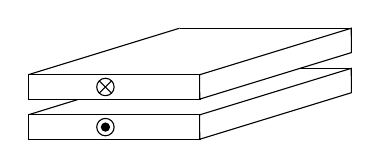
\begin{tikzpicture}[x=0.75pt,y=0.75pt,yscale=-1,xscale=1]
%Straight Lines  
\draw    (354.84,100.73) -- (413.03,100.73) ;
%Straight Lines  
\draw    (257.39,123.13) -- (317.29,104.64) ;
%Shape: Rectangle  
\draw  [fill={rgb, 255:red, 255; green, 255; blue, 255 }  ,fill opacity=1 ] (257.39,123.13) -- (340.15,123.13) -- (340.15,134.93) -- (257.39,134.93) -- cycle ;
%Shape: Rectangle  
\draw  [fill={rgb, 255:red, 255; green, 255; blue, 255 }  ,fill opacity=1 ] (339.97,123.14) -- (413.03,100.73) -- (413.07,112.48) -- (340.01,134.89) -- cycle ;
%Shape: Rectangle  
\draw  [fill={rgb, 255:red, 255; green, 255; blue, 255 }  ,fill opacity=1 ] (257.39,103.8) -- (340.15,103.8) -- (340.15,115.6) -- (257.39,115.6) -- cycle ;
%Shape: Rectangle  
\draw  [fill={rgb, 255:red, 255; green, 255; blue, 255 }  ,fill opacity=1 ] (339.97,103.81) -- (413.03,81.4) -- (413.07,93.15) -- (340.01,115.55) -- cycle ;
%Flowchart: Summing Junction  
\draw   (290.39,109.7) .. controls (290.39,107.39) and (292.27,105.51) .. (294.58,105.51) .. controls (296.9,105.51) and (298.77,107.39) .. (298.77,109.7) .. controls (298.77,112.01) and (296.9,113.89) .. (294.58,113.89) .. controls (292.27,113.89) and (290.39,112.01) .. (290.39,109.7) -- cycle ; \draw   (291.62,106.74) -- (297.54,112.66) ; \draw   (297.54,106.74) -- (291.62,112.66) ;
%Shape: Ellipse  
\draw   (290.39,129.03) .. controls (290.39,126.72) and (292.27,124.85) .. (294.58,124.85) .. controls (296.9,124.85) and (298.77,126.72) .. (298.77,129.03) .. controls (298.77,131.35) and (296.9,133.22) .. (294.58,133.22) .. controls (292.27,133.22) and (290.39,131.35) .. (290.39,129.03) -- cycle ;
%Shape: Ellipse  
\draw  [fill={rgb, 255:red, 0; green, 0; blue, 0 }  ,fill opacity=1 ] (292.64,129.03) .. controls (292.64,127.96) and (293.51,127.09) .. (294.58,127.09) .. controls (295.66,127.09) and (296.53,127.96) .. (296.53,129.03) .. controls (296.53,130.11) and (295.66,130.98) .. (294.58,130.98) .. controls (293.51,130.98) and (292.64,130.11) .. (292.64,129.03) -- cycle ;
%Straight Lines  
\draw [fill={rgb, 255:red, 255; green, 255; blue, 255 }  ,fill opacity=1 ]   (257.39,103.8) -- (324.11,83.29) -- (330.27,81.4) ;
%Straight Lines  
\draw [fill={rgb, 255:red, 255; green, 255; blue, 255 }  ,fill opacity=1 ]   (330.27,81.4) -- (413.03,81.4) ;
\end{tikzpicture}

{\renewcommand*{\arraystretch}{0.2}
    \begin{tabularx}{0.5\columnwidth}{|X|}
        \hline
        \[R=\frac{2}{w\delta\sigma}\] \\
        \hline
        \[L=\frac{\mu d}{w}\]         \\
        \hline
        \[G=\frac{\sigma w}{d}\]      \\
        \hline
        \[C=\frac{w\varepsilon}{d}\]  \\
        \hline
    \end{tabularx}}

\vspace{1ex}
Für beliebige Leitergeometrie gelten folgende Zusammenhänge:
\[
    LC = \mu\varepsilon \quad \text{und} \quad \frac{G}{C} = \frac{\sigma}{\varepsilon}
\]

\subsection{Allgemeine Lösung Leitungsgleichung}
\begin{align*}
    U(z) & = U^+ e^{\gamma z} + U^- e^{-\gamma z} = U^+ e^{\gamma d} + U^ - e^{-\gamma d}                      \\
    I(z) & = I^+ e^{\gamma z} + I^- e^{-\gamma z} = \frac{U^+}{Z_L}e^{\gamma d} - \frac{U^-}{Z_L}e^{-\gamma d} \\
    Z_L  & = \frac{U^+}{I^+} = \sqrt{ \frac{R + j \omega L}{G + j \omega C}}
\end{align*}

\begin{align*}
    \gamma      & = j \omega \sqrt{LC} \cdot \sqrt{ \frac{RG}{j^2 \omega^2 LC} + \frac{G}{j \omega C} + \frac{R}{j \omega L} + 1}                             \\
    \lambda     & = \frac{2 \pi}{\beta}                                                                                                                       \\
    v_{Ph}      & = \frac{\omega}{\beta}                                                                                                                      \\
    l_{elektr.} & = \beta \cdot l                                                                                                                             \\
    \alpha      & = \omega \cdot \sqrt{\dfrac{\mu \varepsilon}{2}\cdot \left(\sqrt{1+\dfrac{\sigma^2}{\omega^2\cdot\varepsilon^2}}{\color{red}{-}}1\right)}   \\
    \beta       & = \omega \cdot \sqrt{\dfrac{\mu \varepsilon}{2}\cdot \left(\sqrt{1+\dfrac{\sigma^2}{\omega^2\cdot\varepsilon^2}}{\color{green}{+}}1\right)}
\end{align*}

\subsubsection{Verlustlose Übertragungsleitung}
\begin{align*}
    \underline{\gamma} & = j\omega\sqrt{LC}= j\beta                                                                                           \\
    Z_L                & =\frac{U^+}{U^-}       = \sqrt{\frac{L}{C}}                                                                          \\
    v                  & = \frac{\omega}{\beta} = \frac{1}{\sqrt{LC}}= \frac{1}{\sqrt{\mu\varepsilon}}= \frac{c_0}{\sqrt{\mu_r\varepsilon_r}} \\
    \lambda            & = \frac{2\pi}{\beta}=\frac{1}{f\sqrt{LC}}= \frac{v}{f}= \frac{c_0}{f\sqrt{\mu_r\varepsilon_r}}
\end{align*}

\subsubsection{vernachlässigbarer Widerstandsbelag}
\includegraphics[width=\columnwidth]{Figures/vernachlaessigbarerWiderstandsbelag.png}


\subsubsection{vernachlässigbarer Leitwertbelag}
\includegraphics[width=\columnwidth]{Figures/vernachlaessigbarerLeiterwertbelag.png}

\subsection{Übertragungsleitung mit Last}

\resizebox{0.4\textwidth}{!}{
    \begin{tikzpicture}
        \begin{circuitikz}%[american voltages]
            %Schaltbild
            \draw(0,0)
            to[V,v=$u_G(t)$](0,2)                               %Spannungsquelle
            to[R=$Z_g$](2,2)                                    %Quelleninnenwiderstand
            to[short,o-o](6,2)                                  %Leitung mit Knoten
            to[short](8 ,2)
            to[R= $Z_A$](8,0)                                   %Lastwiderstand
            to[short](6,0)                                      
            to[short,o-o](2,0)                                  %Leitung mit Knoten
            to[short](0,0);   
            
            %linke gestrichelte linie
            \draw[dotted](2,0)--(2,-0.5) node[left]{$l=0$};
            \draw[dotted](2,-0.5)--(2,-1) node[left]{$z=d$};
            \draw[dotted](2,-1)--(2,-1.5);

            %Pfeil in richtung l
            \draw[->](2,-0.5) -- (6,-0.5);
            \node at (3,-0.5)[above]{positiv $l$};
            
            %rechte gestrichelte Linue
            \draw[dotted](6,0)--(6,-0.5) node[right]{$l=d$};          
            \draw[dotted](6,-0.5)--(6,-1) node[right]{$z=0$};
            \draw[dotted](6,-1)--(6,-1.5);

            %pfeil in richtung z
            \draw[->](6,-1) -- (2,-1);
            \node at (5,-1)[above]{positiv $z$};

            %Pfeil in vorwärts richtung
            \draw[->](2,1.25) -- (5,1.25);
            \node at (3.5,1.25)[above]{hinlaufende Welle};

            %Pfeil in rückwärts richtung
            \draw[->](6,0.5) -- (3,0.5);
            \node at (4.5,0.5)[above]{rücklaufende Welle};
        \end{circuitikz}
    \end{tikzpicture}
}

\begin{align*}
    U(z) & = U^+ e^{\gamma z} + U^- e^{-\gamma z} = U^+ e^{\gamma d} + U^ - e^{-\gamma d}                      \\
    I(z) & = I^+ e^{\gamma z} + I^- e^{-\gamma z} = \frac{U^+}{Z_L}e^{\gamma d} - \frac{U^-}{Z_L}e^{-\gamma d}
\end{align*}

\begin{align*}
    \underline{z}_n & = \frac{\underline{Z}_A}{Z_L}                     & \underline{r} & = \frac{\underline{z}_n-1}{\underline{z}_n+1}= \frac{1-\underline{y}_n}{1+\underline{y}_n} \\
    \underline{r}_A & = \frac{\underline{Z}_A-Z_L}{\underline{Z}_A+Z_L} & m             & = \frac{1-|\underline{r}|}{1+|\underline{r}|}
\end{align*}

\subsubsection{Reflexionsfaktor entlang einer Leitung}
\begin{align*}
    r_E    & = r_A  ^{-2\gamma l} = r_A  e^{-2\alpha l} e^{-j2\beta l}                                                     \\
    \alpha & = -\frac{\ln(r_A)}{2l} [\si{Np/m}]                        & \beta & = \dfrac{\phi_2 -\phi_1}{2l} [\si{rad/m}]
\end{align*}

\subsubsection{Stehwellenverhältnis}
\begin{align*}
    \mathrm{SWR} = \frac{U_\text{max}}{U_\text{min}} =
    \frac{I_\text{max}}{I_\text{min}} = \frac{1+|r(z)|}{1-|r(z)|} =
    \frac{|U_H|+|U_R|}{|U_H|-|U_R|}
\end{align*}

\subsubsection{Position von Extrema}
\begin{align*}
    \Aboxed{r_A & = |r_A|\cdot e^{-j\theta_r}}\rightarrow\theta_r\text{ in rad}                                 \\
    z_{min}     & =\frac{\lambda}{4\pi}(\theta_r+(2n+1)\cdot\pi)\rightarrow\text{Minima alle }\frac{\lambda}{2} \\
    z_{max}     & =\frac{\lambda}{4\pi}(\theta_r+2n\pi)\rightarrow\text{Maxima alle }\frac{\lambda}{2}
\end{align*}

\subsubsection{Spezialfall: Angepasste Leitung}
\begin{align*}
    Z_A  & = Z_L = Z(z)                              \\
    r_A  & = 0\qquad\rightarrow\text{reflexionsfrei} \\
    SWR  & = 1                                       \\
    U(z) & = U^+\cdot e ^{j\beta z}                  \\
    I(z) & = I^+ \cdot e^{j\beta z}                  \\
         & = \frac{U^+}{Z_L}\cdot e^{j\beta z}
\end{align*}

\subsubsection{Spezialfall: Kurzgeschlossene Leitung}
\begin{align*}
    Z_A  & = 0                                                                        \\
    Z(z) & = j Z_L\cdot\tan(\beta z)        \qquad\rightarrow\text{rein imaginär}     \\
    r_A  & = -1                                                                       \\
    SWR  & = \infty                                                                   \\
    U(z) & = U^+\cdot 2j\sin(\beta z)    \qquad\rightarrow U(z=0)=0                   \\
    I(z) & = U^+\cdot 2\cos(\beta z)    \qquad\rightarrow I(z=0)=I_A=\frac{2U^+}{Z_L}
\end{align*}

\subsubsection{Spezialfall: Leerlaufende Leitung}
\begin{align*}
    Z_A  & = \infty                                                                   \\
    Z(z) & = -jZ_L\cdot \cot(\beta z) \qquad\rightarrow\text{rein imaginär}           \\
    r_A  & = 1                                                                        \\
    SWR  & = \infty                                                                   \\
    U(z) & = U^+\cdot 2\cos(\beta z) \qquad\rightarrow U(z=0)=0                       \\
    I(z) & = U^+\cdot 2j\sin(\beta z) \qquad\rightarrow I(z=0)=I_A = \frac{2U^+}{Z_L}
\end{align*}

\subsubsection{Spezialfall: Ohm'sch abgeschlossene Leitung}
\[
    r_A = \texttt{reell}
\]

\begin{align*}
    \underline{R_A > Z_L} & \rightarrow\theta_r = 0                      \\
                          & \rightarrow z_{max}=\frac{\lambda}{2}\cdot n
\end{align*}

\begin{align*}
    \underline{R_A < Z_L} & \rightarrow\theta_r = \pi                    \\
                          & \rightarrow z_{min}=\frac{\lambda}{2}\cdot n
\end{align*}

\subsection{Mehrfachreflexionen bei fehlender Anpassung}

\tikz{
    %Linien
    \draw[-] (1,0) -- (1,6);
    \draw[-] (5,0) -- (5,6);

    %Pfeile mit Bezeichnungen
    \draw[->] (3.5,6.5) -- (5,6.5)node[right]{$z$};

    \draw[->] (1,6) -- (5,5) node[right]{$t_D$};
    \draw[-] (1,6) -- (3,5.5) node[above]{$U_{1h}$};

    \draw[->] (5,5) -- (1,4)node[left]{$2t_D$};
    \draw[-] (5,5) -- (3,4.5) node[above]{$U_{1r}$};

    \draw[->] (1,4) -- (5,3)node[right]{$3t_D$};
    \draw[-] (1,4) -- (3,3.5) node[above]{$U_{2h}$};

    \draw[->] (5,3) -- (1,2)node[left]{$4t_D$};
    \draw[-] (5,3) -- (3,2.5) node[above]{$U_{2r}$};

    \draw[->] (1,2) -- (5,1)node[right]{$5t_D$};
    \draw[-] (1,2) -- (3,1.5) node[above]{$U_{3h}$};

    
    \draw[dotted ] (5,1) -- (3,0.5);

    %Klammern mit Bezeichnungen
    \draw [black,
        decorate,
        decoration = {brace,
                raise=5pt,
                amplitude=5pt}] (1,4.2) --  (1,5.8);
    \draw[] (0.5,5) -- (0.5,5) node[left]{$U_{1h}$};

    \draw [black,
        decorate,
        decoration = {brace,
                raise=5pt,
                amplitude=5pt}] (5,4.8) --  (5,3.2);
    \draw[] (5.5,4) -- (5.5,4) node[right]{$U_{1h}(1+r_A)$};

    \draw [black,
        decorate,
        decoration = {brace,
                raise=5pt,
                amplitude=5pt}] (1,2.2) --  (1,3.8);
    \draw[] (0.5,3) -- (0.5,3) node[left]{$U_{1h}$};
    \draw[] (0.5,2.5) -- (0.5,2.5) node[left]{$+(1+_I)U_{1r}$};

    \draw [black,
        decorate,
        decoration = {brace,
                raise=5pt,
                amplitude=5pt}] (5,2.8) --  (5,1.2);
                \draw[] (5.5,2) -- (5.5,2) node[right]{$U_{1h}(1+r_A)$};
                \draw[] (5.5,1.5) -- (5.5,1.5) node[right]{$+U_{2h}(1+r_A)$};


    \draw [black,
        decorate,
        decoration = {brace,
                raise=5pt,
                amplitude=5pt}] (1,0.2) --  (1,1.8);
    \draw[] (0.5,1.5) -- (0.5,1.5) node[left]{$U_{1h}$};
    \draw[] (0.5,1) -- (0.5,1) node[left]{$+(1+r_I)U_{1r}$};
    \draw[] (0.5,0.5) -- (0.5,0.5) node[left]{$+(1+r_I)U_{2r}$};

}
\begin{align*}
    U_{1h} & = \frac{U_G\cdot Z_L}{R_I + Z_L}            \\
    U_{1r} & = r_A\cdot U_{1h}                           \\
    U_{2h} & = r_I\cdot U_{1r} = r_I\cdot r_A U_{1h}     \\
    U_{2r} & = r_A\cdot U_{2h} = r_I\cdot r_A^2 U_{1h}   \\
    U_{3h} & = r_I\cdot U_{2r} = r_I^2\cdot r_A^2 U_{1h}
\end{align*}
\resizebox{0.4\textwidth}{!}{
    %\centering
    \begin{tikzpicture}
        \begin{circuitikz}%[american voltages]
            \draw(0,0)
            to[V,v=$u_G(t)$](0,2)   %Spannungsquelle
            to[R=$R_I \neq Z_L$](2,2) %Quelleninnenwiderstand
            to[short](8,2)
            to[R= $R_A\neq Z_L$](8,0)
            to[short](0,0)
            (4,2) to [open, v=$u(z\mathpunct{,}t)$] (4,0) %Spannungspfeil u(z,t)
            (2,2) to [open, v=$u_E(t)$] (2,0) %Spannungspfeil u_E(t)
            (6,2) to [open, v=$u_A(t)$] (6,0); %Spannungspfeil u_A(t)
            \draw[-] (2,2) circle (0.1);
            \draw[-] (6,2) circle (0.1);
            \draw[-] (2,0) circle (0.1);
            \draw[-] (6,0) circle (0.1);
        \end{circuitikz}
    \end{tikzpicture}
}
